\section{Computational Models}

The model of choice for representing the post-synaptic potential (PSP) we chose to work with is a double exponential function, given as follows:

\begin{equation}
    v(t) = v_0 \cdot (e^{-t/\tau_m} - e^{-t/\tau_s})
\end{equation}

The choice of this model is grounded on several key considerations. Firstly, the model incorporates two time constants, $\tau_m$ and $\tau_s$, enabling the simulation of both the rise and decay dynamics of the neuronal response. The $\tau_m$ parameter corresponds to the membrane time constant, responsible for governing the rise time of the response, while $\tau_s$ associates with the synaptic time constant, determining the width of the spike response.

These temporal dynamics afford an opportunity to distinguish patterns in the data set that might not be discernible with other models harboring a single time constant. For example, if two input spikes are close together, the neuron's response to the second spike will be influenced by the residual effect of the first spike. Such an effect can prove crucial for the recognition of patterns in data sets wherein input spike times exhibit complex correlations.

\subsection{Spike Response Peak}

\begin{mdframed}[backgroundcolor=red_background, linecolor=black, linewidth=2pt, frametitle=\textbf{Statement}]
\begin{center}

    \label{st:peak}
    The time at which the neuron's response peaks, $t_{peak}$, is given by

    
\begin{equation}
t_{peak} = \frac{\tau_m \tau_s}{\tau_m - \tau_s} \ln\left(\frac{\tau_m}{\tau_s}\right)
\end{equation}

\end{center}
\end{mdframed}

\textbf{Proof:}
The derivative of $v(t)$ is:

\begin{equation}
v'(t) = v_0 \cdot \left(\frac{-e^{-t/\tau_m}}{\tau_m} + \frac{e^{-t/\tau_s}}{\tau_s}\right)
\end{equation}

Setting $v'(t) = 0$ and solving for $t$ results in:

\begin{equation}
0 = \frac{-e^{-t/\tau_m}}{\tau_m} + \frac{e^{-t/\tau_s}}{\tau_s}
\end{equation}

\begin{equation}
v'(t) = v_0 \cdot \left(\frac{-e^{-t/\tau_m}}{\tau_m} + \frac{e^{-t/\tau_s}}{\tau_s}\right)
\end{equation}

Setting $v'(t) = 0$, we obtain:

\begin{equation}
0 = \frac{-e^{-t/\tau_m}}{\tau_m} + \frac{e^{-t/\tau_s}}{\tau_s}
\end{equation}

Rearranging the terms gives us:

\begin{equation}
\frac{e^{-t/\tau_m}}{\tau_m} = \frac{e^{-t/\tau_s}}{\tau_s}
\end{equation}

Taking natural logarithms on both sides, we have:

\begin{equation}
\frac{t}{\tau_m} - \ln \tau_m = - \frac{t}{\tau_s} - \ln \tau_s
\end{equation}

Rearranging terms again:

\begin{equation}
t \left( \frac{1}{\tau_s} - \frac{1}{\tau_m} \right) = \ln \tau_m - \ln \tau_s = \ln\left(\frac{\tau_m}{\tau_s}\right)
\end{equation}

Solving for $t$ yields:

\begin{equation}
t_{peak} = \frac{\tau_m \tau_s}{\tau_m - \tau_s} \ln\left(\frac{\tau_m}{\tau_s}\right)
\end{equation}


\subsection{Response Width}

The spike response width, $W_{spike}$, can be computed by finding the times at which the neuron's response reaches a certain fraction of the peak response (denoted as $\alpha_{cut}$). If we denote these times as $t_1$ and $t_2$, the spike response width is given by $W_{spike} = t_2 - t_1$.

\begin{mdframed}[backgroundcolor=red_background, linecolor=black, linewidth=2pt, frametitle=\textbf{Statement}]
\begin{center}

    \label{st:window-width}
    For $\alpha_{cut} = \frac{1}{10}$ the spike response width, $W_{spike}$, approximates to:

    \begin{equation}
        W_{spike} \approx \tau_m \ln(10)
    \end{equation}

\end{center}
\end{mdframed}


\textbf{Proof:}

For $\alpha_{\text{{cut}}} = \frac{1}{10}$ we need to find the solutions to the equation
\begin{equation}
    v(t) = v(t_{\text{{peak}}})/10
\end{equation}
i.e.,
\begin{equation}
e^{-t/\tau_m} - e^{-t/\tau_s} = \frac{1}{10}\left(e^{-t_{\text{{peak}}}/\tau_m} - e^{-t_{\text{{peak}}}/\tau_s}\right)
\end{equation}

Assuming $\tau_m \gg \tau_s$, we can neglect the $e^{-t/\tau_s}$ term in the equation, which gives

\begin{equation}
e^{-t/\tau_m} = \frac{1}{10} e^{-t_{\text{{peak}}}/\tau_m}
\end{equation}

Taking the natural logarithm of both sides, we get:

\begin{equation}
-t/\tau_m = \ln(1/10) - t_{\text{{peak}}}/\tau_m
\end{equation}

Solving for $t$ yields:

\begin{equation}
t = t_{\text{{peak}}} - \tau_m \ln(10)
\end{equation}

As $t_{\text{{peak}}}$ is the point at which the neuron's response peaks, the time at which the neuron's response is one-tenth of the peak response (i.e., the width of the spike) is $t_1 = t_{\text{{peak}}} + \tau_m \ln(10)$.

Thus, the spike width $W_{\text{{spike}}}$ is given by:

\begin{equation}
W_{\text{{spike}}} \approx t_1 - t_{peak} = \tau_m \ln(10)
\end{equation}

Under the assumption that $\tau_m >> \tau_s$, this result is consistent with the understanding that the spike width would be dominated by the membrane time constant $\tau_m$. 

For example, for $\tau_m = 15$ ms and $\tau_s = \tau_m / 4 = 3.75$ ms, we can calculate the spike width $W_{\text{{spike}}}$ using the formula obtained earlier:

\begin{equation}
W_{\text{{spike}}} = \tau_m \ln(10)
\end{equation}

Substitute $\tau_m = 15$ ms into the equation, we get:

\begin{equation}
W_{\text{{spike}}} = 15 \times \ln(10) \approx 34.54 \text{ ms}
\end{equation}

With the parameters $\tau_m$ and $\tau_s$ granting control over both the rise time and the response width, this model becomes an ideal tool for understanding neural coding in a broad range of scenarios.

\begin{figure}[H]
    \centering
    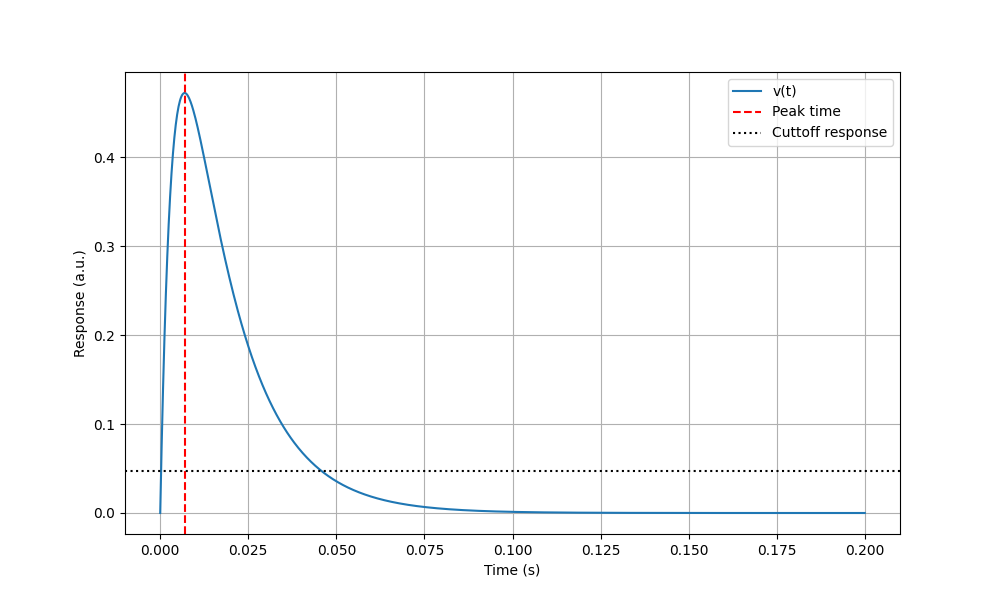
\includegraphics[width=0.5\linewidth]{methods//computational-models//graphs/model_analysis.png}
    \caption{Double Exponent with $\tau_m=15ms$ and $\tau_s=\frac{\tau_m}{4}$ }
    \label{fig:exm-double-exp}
\end{figure}